\chapter{Matrice de vérification des performances}
Ce chapitre présente les performances réelles obtenues au moyen des simulations présentées dans ce rapport. Cette matrice permet de valider l'atteinte des critères présentés dans le cahier des charges. Il est à noter que les simulations n'ont pas toutes été implantées dans le simulateur d'OPAL-RT, pour des raisons de livraison et d'installation.
\begin{figure}[htb]
\centering
\makebox[\textwidth][c]{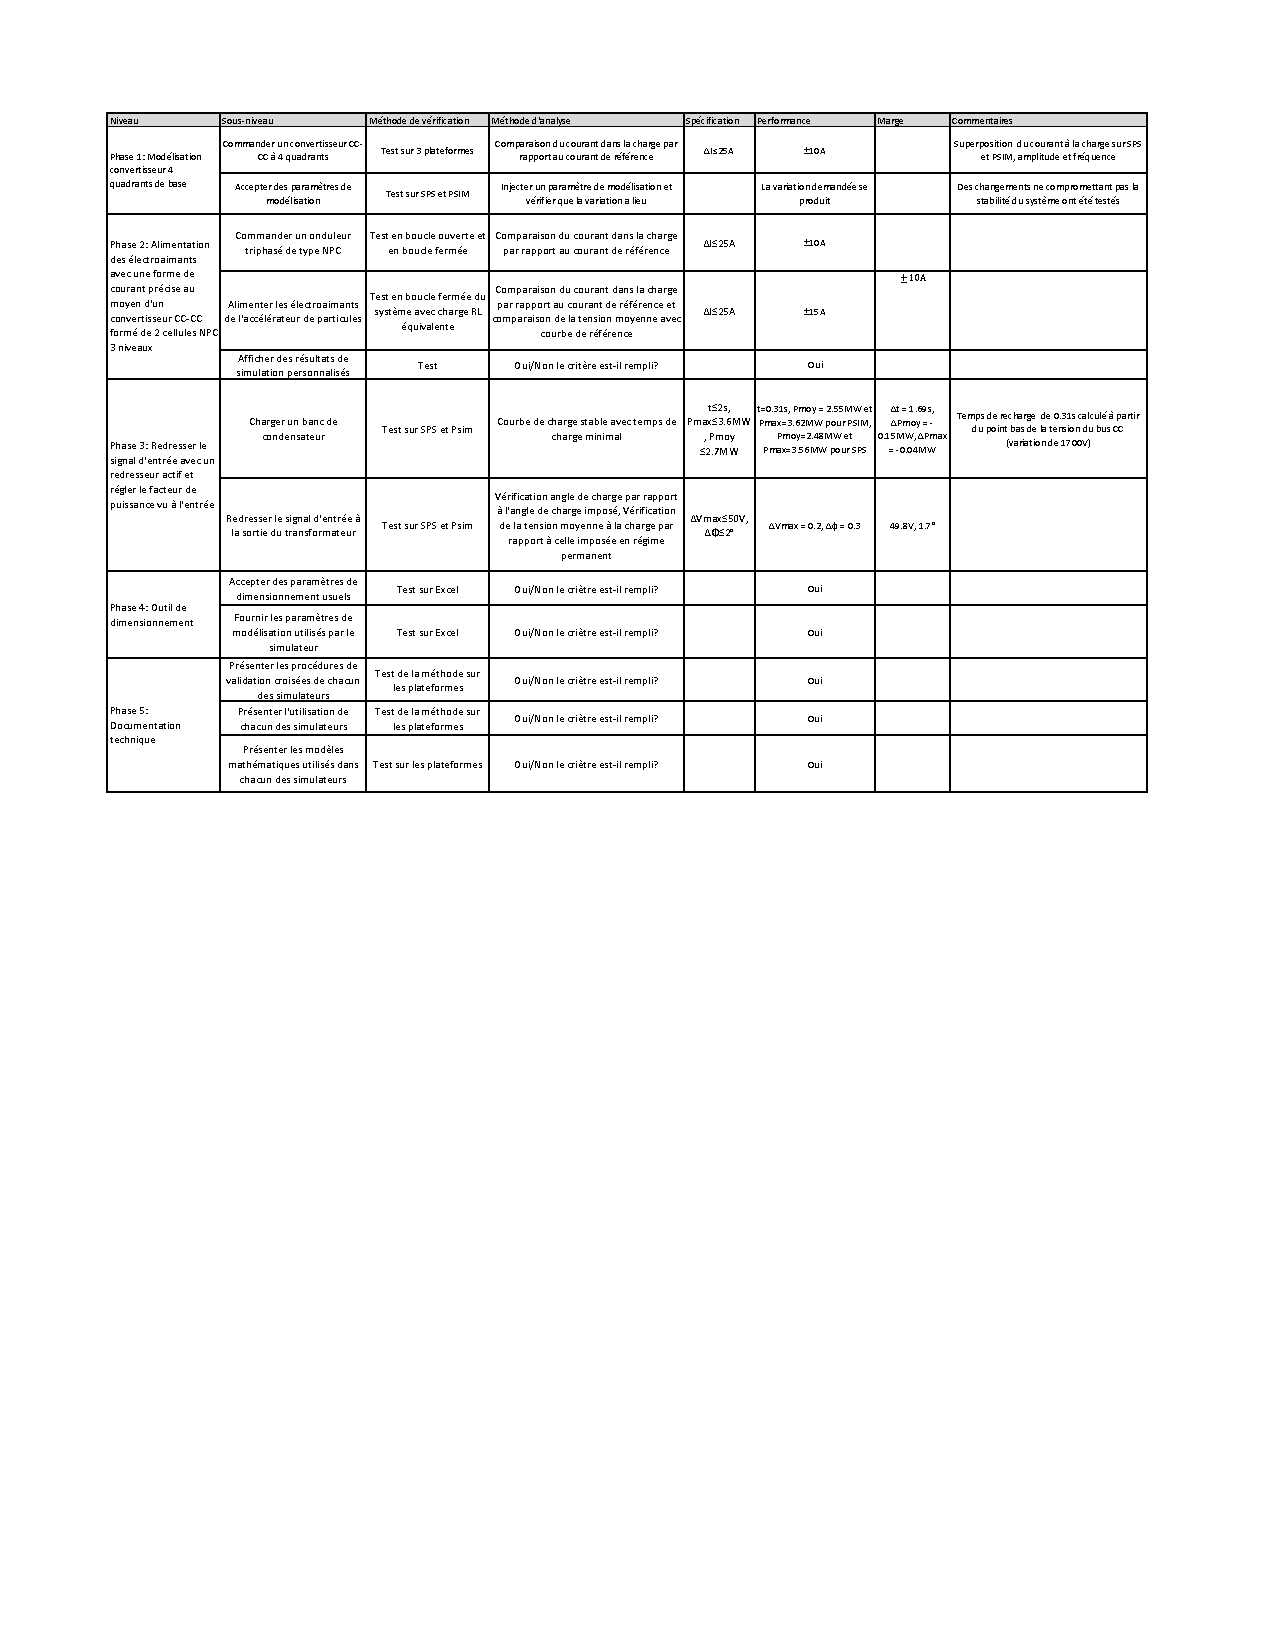
\includegraphics[scale=0.9,trim= 0mm 12cm 0mm 0mm, clip ]{matrice_verification.pdf}}
\caption{Matrice de vérification des performances}
\label{matrice}
\end{figure}